\chapter{Ising model at negative temperatures}
\label{ch:ising}
In this last section I move the focus towards the the study of a more complex model, namely the Ising model. \\
After a brief introduction on the 2D Ising model, I will move towards the description of the simulations. The results of the
simulations are then presented and discussed according to what said in the previous chapters. \\

\section{The Ising model}
The Ising model is a mathematical model initially used to describe magnetic properties of materials in statistical mechanics. It consists in a collection of spins 
organised in a lattice that can assume two values, either 1 or -1. \\
The spins are allowed to interact with their neirest neighbors and in the most general form the hamiltonian assumes the form
\begin{equation}
    \mathcal{H}(\{\sigma_k\}) = -\sum_{\langle i j\rangle} J_{i j} \sigma_{i} \sigma_{j} - \sum_{j} B_j\sigma_{j}
    \label{eq:general_hamiltonian_Ising}
\end{equation}
where $B_j$ indicates the intensity of the magnetic field on the spin $j$ and $J_{ij}$ indicates the strength of the interaction between the spin $i$ and the spin $j$.
In the following analysis I will assume $J_{ij} = J, B_j = B \ \forall i,j$. \\
The sign of the interaction parameter $J$ determines whether we are dealing with ferromagnetic materials ($J>0$) or paramagnetic materials ($J < 0$). In the case of $J=0$
we return to the two levels system discussed in chapter \ref{ch:TLS}. \\
Let us first restrict the analysis to the purely interacting case setting $B=0$. In this case the hamiltonian initially given by \ref{eq:general_hamiltonian_Ising} becomes
\begin{equation*}
    \mathcal{H}(\{\sigma_k\}) = -J \sum_{\langle i j\rangle}\sigma_{i} \sigma_{j}
\end{equation*}
At fixed temperature $T$ the probability of a state is given by the Boltzmann factor
\begin{equation}
    p(\{\sigma_k\}) = \frac{e^{-\beta\mathcal{H}(\{\sigma_k\})}}{Z}
    \label{eq:Boltzmann_factor_Ising}
\end{equation}
where $\beta = \frac{1}{k_BT}$ and $Z$ is the canonical partition function
\begin{equation*}
    Z(\beta, V, N) = \sum_{\{\sigma_k\}} e^{-\beta\mathcal{H}(\{\sigma_k\})}
\end{equation*}
Let us consider the probability factor \ref{eq:Boltzmann_factor_Ising}, which explicitly becomes 
\begin{equation*}
    p(\{\sigma_k\}) \propto e^{-\beta J \sum_{\langle i j\rangle}\sigma_{i} \sigma_{j}}
\end{equation*}
and let us define a new new parameter $\xi = \beta J$ so that 
\begin{equation}
    p(\{\sigma_k\}) \propto e^{-\xi \sum_{\langle i j\rangle}\sigma_{i} \sigma_{j}}
    \label{eq:probability_Ising}
\end{equation}

\subsubsection*{Ferromagnetic systems}
In the ferromagnetic case $J > 0$, hence $\xi > 0$. For $\xi \to 0$, which can be either a high temperature or a weak coupling, one can see that 
$p(\{\sigma_k\}) \to 1$ independently on the values $\sigma_k$ so that we expect the spins to be almost evenly distributed between up and down. \\
Instead for $\xi \to +\infty$ which can be either a low temperature or a strong coupling, one has that the exponential in \ref{eq:probability_Ising} except when
$\sum_{\langle i j\rangle}\sigma_{i} \sigma_{j}$ is close to zero, hence we expect, again, the spins to be evenly distributed between up and down.
\subsubsection*{Paramagnetic systems}
In this case $J > 0$, hence $\xi > 0$. For $\xi \to 0$ the result is the same as for ferromagnetic systems. \\
When $\xi \to -\infty$ the exponential factor in \ref{eq:probability_Ising} grows indefinetely if $\sum_{\langle i j\rangle}\sigma_{i} \sigma_{j} > 0$, that is when the spins are aligned.
Thus no preference is given to the configuration in which two neighbor spins are aligned both up or down, and we expect it to depend on the history of the system. \\

The study is carried in a 2D lattice which is of the shape reported in figure \ref{fig:IsingLattice}.
\begin{figure}[htbp]
    \centering
    \begin{tikzpicture}
        \foreach \x in {-3,-2,...,3}{
        \foreach \y in {-3,-2,...,3}{
            \draw [->] (\x,\y-0.15) -- (\x,\y+0.15);
        }
      }
    \end{tikzpicture}
    \caption{}
    \label{fig:IsingLattice}
\end{figure}
Let us focus the attention on a $2x2$ subset of the lattice. The possible energies are 
\begin{align*}
    \begin{pmatrix} \uparrow & \uparrow \\ \uparrow & \uparrow \end{pmatrix}_1 \ E = 4J \\
    \begin{pmatrix} \downarrow & \uparrow \\ \uparrow & \uparrow \end{pmatrix}_1 \ E = 4J \\
    \begin{pmatrix} \downarrow & \downarrow \\ \uparrow & \uparrow \end{pmatrix}_1 \ E = 4J \\
    \begin{pmatrix} \downarrow & \downarrow \\ \downarrow & \uparrow \end{pmatrix}_1 \ E = 4J
\end{align*}
\begin{align*}
    &\begin{pmatrix} &\uparrow&\\ \uparrow&\uparrow&\uparrow\\ &\uparrow&\\\end{pmatrix}_1 \ \Longrightarrow
    \begin{pmatrix} &\uparrow&\\ \uparrow&\downarrow&\uparrow\\ &\uparrow&\\\end{pmatrix}_2 \qquad
    \Delta E = 2J\cdot4 = 8J& \\
    &\begin{pmatrix} &\uparrow&\\ \downarrow&\uparrow&\uparrow\\ &\uparrow&\\\end{pmatrix}_1 \ \Longrightarrow
    \begin{pmatrix} &\uparrow&\\ \downarrow&\downarrow&\uparrow\\ &\uparrow&\\\end{pmatrix}_2 \qquad
    \Delta E = 2J\cdot2 = 4J& \\
    &\begin{pmatrix} &\downarrow&\\ \downarrow&\uparrow&\uparrow\\ &\uparrow&\\\end{pmatrix}_1 \ \Longrightarrow
    \begin{pmatrix} &\downarrow&\\ \downarrow&\downarrow&\uparrow\\ &\uparrow&\\\end{pmatrix}_2 \qquad
    \Delta E = 2J\cdot0 = 0& \\
    &\begin{pmatrix} &\downarrow&\\ \downarrow&\uparrow&\uparrow\\ &\downarrow&\\\end{pmatrix}_1 \ \Longrightarrow
    \begin{pmatrix} &\downarrow&\\ \downarrow&\downarrow&\uparrow\\ &\downarrow&\\\end{pmatrix}_2 \qquad
    \Delta E = 2J\cdot(-2) = -4J& \\
    &\begin{pmatrix} &\downarrow&\\ \downarrow&\uparrow&\downarrow\\ &\downarrow&\\\end{pmatrix}_1 \ \Longrightarrow
    \begin{pmatrix} &\downarrow&\\ \downarrow&\downarrow&\downarrow\\ &\downarrow&\\\end{pmatrix}_2 \qquad
    \Delta E = 2J\cdot(-4) = -8J& \\
\end{align*}

\section{Markov Chain Monte Carlo}
To study the physical properties of the system at equilibrium in a certain macrostate $X$, one needs to perform ensemble averages (er expectation values). The expectation value of a physical quantity $A$ is computed as 
\begin{equation}
    \bar A = \frac{\int A e^{-\beta H} d\tau}{\int e^{-\beta H} d \tau}
    \label{eq:averageval}
\end{equation}
where tha variable $\tau$ runs over all the possible microstates compatible with the given macrostate $X$. \\
Practically speaking, to perform such averages during the simulation, one needs to
\begin{enumerate}
    \item Bring the system in a configuration compatible with specified macrostate 
    \item Calculate the value of the desired quantity in the specific microstate 
    \item Store the value
    \item Move the system to another microstate compatible with the specified macrostate and repeat from point 2 until desired
    \item Perform the average
\end{enumerate}
Of course, in order to perform an accurate average, one needs to 
\begin{enumerate}
    \item Guarantee that the system visit every possible microstate compatible with the macroscopical configuration so that all the possible values of the physical quantity are taken into account when performing the average
    \item Guarantee that every possible state is visited with a frequency that is equal to the probability of the state itself
\end{enumerate}
This can be accomplished by means of the Monte Carlo method, precisely by means of the Metropolis-Hastings algorithm, which allows to perform a random walk trough the configurations of the system and respect the above states conditions under the correct assumptions. \\
The main points of the Metropolis-Hastings' algorithm are now briefly reported, inviting the reader to consult more appropriate sources for further information. \\
Let us suppose that we want to sample from a probability distribution $p(x)$. \\
The system is initially prepared in a certain configuration $x$ which can be arbitrarilly chosen. Each Monte-Carlo cycle then consists in the following steps
\begin{enumerate}
    \item A new configuration of the system $x^*$ is proposed sampling from a proposal distribution $J(x^*|x)$. The proposal distribution can be arbitrarilly chosen, provided the fact that is symmetric $J(x^*|x) = J(x|x^*)$ and that in an infinite number of steps, it guarantees that 
    every states is visited.
    \item The ratio of the probabilities of the two states of the system is then calculated
    \begin{equation*}
        w = \frac{p(x^*)}{p(x)}
    \end{equation*}
    \item if $w \geq 1$ the proposal change is accepted and $x_{i+1} = x^*$
    \item otherwise a number $r$ is extracted from a uniform distribution in $[0,1]$. If $w > r$ the proposal change is still accepted and $x_{i+1} = x^*$. Otherwise the proposal moved is refused and $x_{i+1} = x_i$
\end{enumerate}
The higher the number of Monte-Carlo cycles, the closer is the distribution of the visited states to the probability distribution $p(x)$, the more precise the expectation values calculated as \ref{eq:averageval}. \\
Practically speaking the simplest choice for the proposal distribution $J(x^*|x)$, even if not the most efficient, is the uniform distribution. The distribution $p(x)$, on the other side, is related to the ensemble 
in which we describe the system: in the canonical ensemble $p(x)$ is given by the Maxwell-Boltzmann distribution given in equation \ref{eq:Boltzmann_factor_Ising}.
\footnote{Difference between Metropolis and Metropolis-Hastings}

\section{Single system at negative temperature}
The first case I want to study is one single system prepared at temperature $T$. In order to perform the simulation, the system is initially prepared in a random configuration: then the systems goes under $10^7$ Monte Carlo cycles 
sampling from the probability distribution given by \ref{eq:Boltzmann_factor_Ising}. The simulations are run for three different values of the temperature, that is $T_1 = \SI{0}{\kelvin}, T_2 = \SI{1}{\kelvin}, T_3 = \SI{1000}{\kelvin}$, and each of them is run both 
for the ferromagnetic antiferromagnetic cases. \\
Figure \ref{fig:MC_single_final_state_ferro} reports the final state of a ferromagnetic system, while
figure \ref{fig:MC_single_final_state_antiferro} reports those of an antiferromagnetic system for the same temperature values.
\begin{figure}
    \centering 
    \caption{}
    \label{fig:MC_single_final_state_ferro}
\end{figure}
\begin{figure}
    \centering 
    \caption{}
    \label{fig:MC_single_final_state_antiferro}
\end{figure}
\section{Two systems into contact}
Two systems are prepared at temperature $T_1$ and $T_2$. The spin configurations are obtained after $10^4$ Monte Carlo cycles in the canonical ensemble. \\
After that, the two systems are put into contact forming a new system that can be threated as a microcanonical ensemble. The simulation of the latter was obtained with a 
demon Monte Carlo method with $10^6$ cycles.

\begin{figure}[htbp]
    \centering
    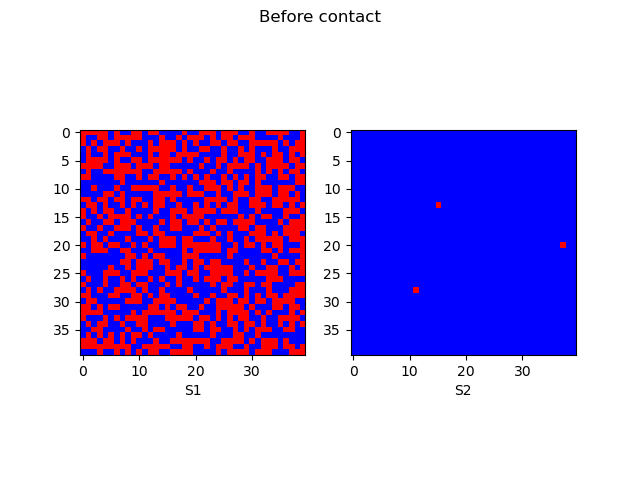
\includegraphics[scale=0.7]{./images/T1_T2_before.png}
    \caption{Before contact}{The red tiles indicate the \emph{up} state, while the blue tiles indicate the \emph{down} state. Before beeing put into contact
    the two systems are prepared respectively at temperature $k_B T_1 = -\infty \, (10^8)$ and $k_B T_2 = 0^+ \, (10^{-8})$}
    \label{fig:before}
\end{figure}

\begin{figure}[htbp]
    \centering
    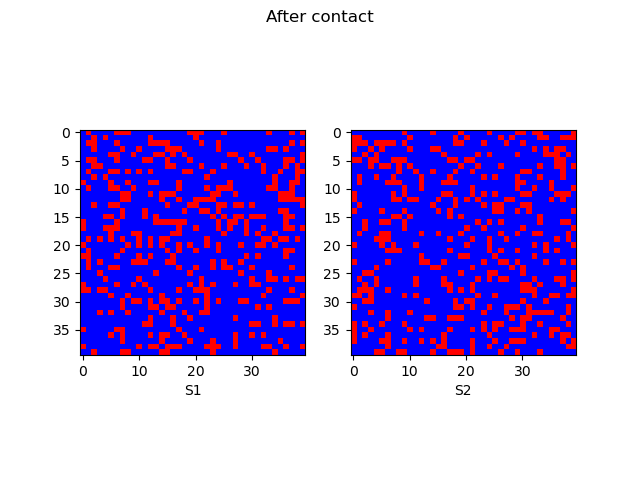
\includegraphics[scale=0.7]{./images/T1_T2_after.png}
    \caption{After contact}{The red tiles indicate the \emph{up} state, while the blue tiles indicate the \emph{down} state. The equilibrium temperature after putting the two systems into contact is in between the two values according to the hierarchy presented 
    at the end of chapter \ref{ch:temperature}. The system at negative temperature get cooled down changing some up states to down states, while the system at positive temperature
    gets heated changing some down states into up. The resuls is of course an approximately equal concentrarion of up/down in both systems.}
    \label{fig:after}
\end{figure}